\newpage

\section{Zufallsgröße und Wahrscheinlichkeitsverteilung}
Muss sich seperrat angeschaut werden script unbrauchbar.
\begin{align}
    x &=\textrm{sei ...}&  x&=x_i & P(X=x_i)
\end{align}
$\longrightarrow$ Würfel $2\times $ werfen, 6 oder keine 6\\
$\longrightarrow$ $2\times 6$ 10€ Gewinn $2\times \overline{6}$ 0€ Gewinn sonst 5€ Gewinn.\\

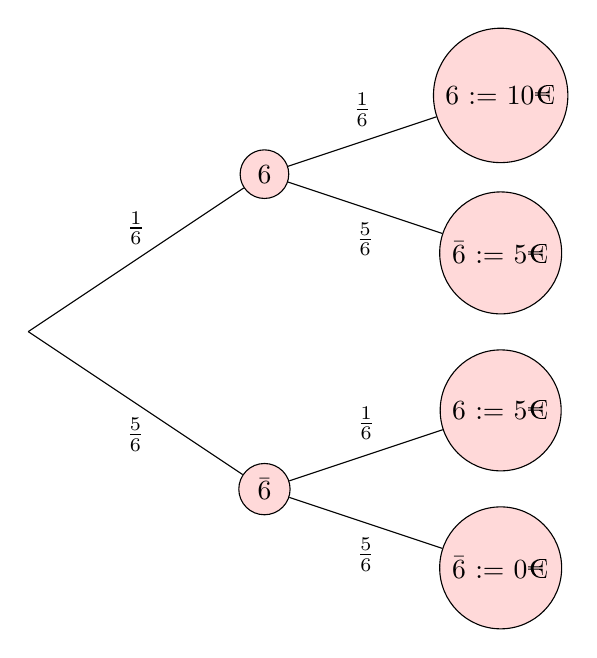
\begin{tikzpicture}[
    circ/.style={draw=black,fill=red!15,circle},
    grow=right,
    level 1/.style={sibling distance=4cm},
    level 2/.style={sibling distance=2cm},
    level distance=3cm]
 \node [coordinate] {}
   child {
     node[circ] {$\bar{6}$}
       child { node[circ] {$\bar{6}$ := 0€}
         edge from parent
         node [below=2] {$\frac{5}{6} $}}
       child { node[circ] {$6$ := 5€}
         edge from parent
         node [above=2] {$\frac{1}{6}$}}
     edge from parent
     node [below=2] {$\frac{5}{6}$}
     }
   child {
     node[circ] {$6$}
       child { node[circ] {$\bar{6}$ := 5€}
         edge from parent
         node [below=2] {$\frac{5}{6}$}}
       child { node[circ] {$6$ := 10€}
         edge from parent
         node [above=2] {$\frac{1}{6}$}
   }
    edge from parent
    node [above=2] {$\frac{1}{6}$}
   };
 \end{tikzpicture}

 \begin{table}[ht]
    \begin{tabular}{llll}
    \textbf{}                       & $x_1$ & $x_2$      & $x_3$ \\
    \multicolumn{1}{l|}{$x=x_i$}    & 10    & 5          & 0     \\ \hline
    \multicolumn{1}{l|}{$P(x=x_i)$} & $\frac{1}{36}$       & $\frac{10}{36} $ & $\frac{25}{36} $     
    \end{tabular}
    \caption{}
    \label{tab:my-table}
    \end{table}

\subsection{Zähldichte}

Muss sich seperrat angeschaut werden script unbrauchbar.

\[f_x(t)=P(X=t)\]